\chapter{Systems} \label{chp:systems}
\epigraph{We must be clear that when it comes to atoms, language can be used only as in poetry.}{Niels Bohr}
\begin{figure}[H]
	\centering
	\label{fig:harmonicoscillator}
	\captionsetup[subfigure]{labelformat=empty}
	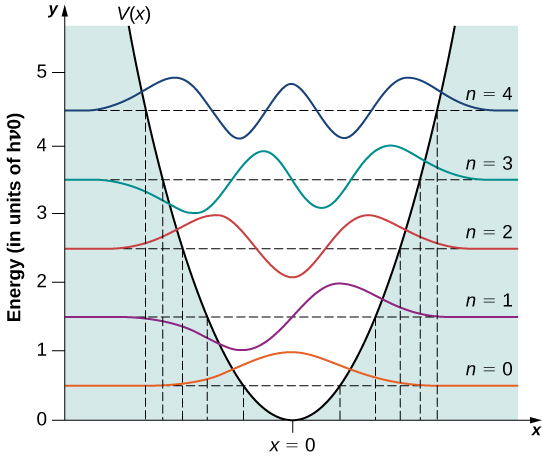
\includegraphics[scale=0.9]{Images/qho.jpg}
	\caption{The quantum harmonic oscillator, with the Hermite functions represented up to 4th order. As in classical mechanics, the harmonic oscillator can describe various quantum systems, such as lattice vibration (phonons) and quantum fields.}
\end{figure}

When defining a system, we also need to specify the basis set to be used. The single particle functions are often known, and they are well-suited as a basis for the total

\section{Quantum dots} \label{subsubsec:quantumdots}
Quantum dots are very small particles, and contain fermions or bosons hold together by an external potential. Since these particles have discrete electronic states like an atom, they are often called artificial atoms. 

In this thesis we will study electrons trapped in harmonic oscillators, which give an external potential affecting particle $i$ is given by
\begin{equation}
u_i=\frac{1}{2}m\omega^2r_i^2.
\end{equation}
Using natural units as described in Appendix B, we can write the Hamiltonian as
\begin{equation}
\label{eq:HOHamiltonian}
\hat{\mathcal{H}} = \sum_{i=1}^{P} \Big(-\frac{1}{2} \nabla_i^2 + \frac{1}{2} r_i ^2\Big) + \sum_{i<j} \frac{1}{r_{ij}} 
\end{equation}
where the energy is scaled with respect to atomic units and lengths are scaled with respect to the Bohr radius.

The exact solutions of the non-interacting Hamiltonian are the Hermite functions, 
\begin{equation}
f_n(x)=H_n(x)\exp(-x^2/2)
\end{equation}
which we will use as our basis. The first four Hermite functions are illustrated in figure \eqref{fig:harmonicoscillator}.

\section{Atomic systems} \label{subsubsec:atomic}
We will also investigate real atoms, which have Hamiltonians defined by the Born-Oppenheimer approximation.

The External potential affecting particle $i$ is therefore
\begin{equation}
u_i=- \frac{1}{2} \frac{Z}{r_i}
\end{equation}


\begin{equation}
\label{eq:AtomicHamiltonian}
\hat{\text{H}} = \sum_{i=1}^{P} (-\frac{1}{2} \nabla_i^2 - \frac{1}{2} \frac{Z}{r_i}) + \sum_{i<j} \frac{1}{r_{ij}},
\end{equation}
which applies for an atom with stationary nucleus at origin. The first part is related to the kinetic energy, while the second is 

"Colloquially, we call such solutions and derived properties as electronic structure."

\section{Molecular systems}

\section{Bose-Einstein Condensation}

\section{Electron gas} \label{subsubsec:electrongas}
\section{Helium gas} \label{subsubsec:heliumgas}
He$^3$ and He$^4$